% The percent symbol creates a comment, which will be ignored by LaTeX when it creates your document.  They're useful for leaving yourself notes and organizing your work.
\documentclass{article}
\usepackage{amsmath, amssymb, tikz} % Required for math symbols
\usepackage[paper=letterpaper,
           hmargin={1in,1in},
           vmargin={1in,1in},
           ]{geometry}   % Allows you to change the margin sizes
\usepackage{enumitem}  % Required to re-label lists

\title{Homework 4}
\author{Xander} 
\date{Mar 3}

\begin{document}

\maketitle
%%%%%%%%%%%%%%%%% Don't delete anything above this line!

\section*{Exercise 5 3.2}  

Prove that every prime number greater than 3 is either one more or one less than a multiple of 6.

\vspace{0.5cm}
\noindent\textbf{Solution Draft:} 
\vspace{0.2cm}

To prove that every prime number greater than 3 is either one more or one less than a multiple of 6, consider the forms an integer \(n\) can take when divided by 6:

\begin{itemize}
    \item \(n = 6k\)
    \item \(n = 6k + 1\)
    \item \(n = 6k + 2\)
    \item \(n = 6k + 3\)
    \item \(n = 6k + 4\)
    \item \(n = 6k + 5\)
\end{itemize}

Analyzing these forms:

\begin{itemize}
    \item \(n = 6k\) is divisible by 6, so it cannot be prime unless \(k=1\), which is not greater than 3.
    \item \(n = 6k + 2 = 2(3k+1)\) and \(n = 6k + 4 = 2(3k+2)\) are even and greater than 2, so they cannot be prime.
    \item \(n = 6k + 3 = 3(2k+1)\) is divisible by 3, and for \(k>0\), \(n\) is greater than 3 and not prime.
\end{itemize}

This leaves us with:

\begin{itemize}
    \item \(n = 6k + 1\) and \(n = 6k + 5 = 6(k+1) - 1\), which are not divisible by 2 or 3.
\end{itemize}

Therefore, any prime number greater than 3 must be in the form of \(6k+1\) or \(6k-1\), showing that it is either one more or one less than a multiple of 6.


%%%%%%%%%%%%%%%%%%%%%%%%%%%%%%%%%%%%
\section*{Exercise 6 3.2}  

What if your \(n\times n\) chessboard is missing two opposite corners? Prove that no matter what \(n\) is, you will not be able to cover the remaining squares with dominoes.

\vspace{0.5cm}
\noindent\textbf{Solution Draft:} 
\vspace{0.2cm}

To prove that an $n \times n$ chessboard with two opposite corners removed cannot be completely covered by dominoes, consider a standard chessboard with an alternating pattern of two colors, typically black and white. A domino, which covers exactly two adjacent squares, will always cover one black square and one white square when placed on the chessboard.

By removing two opposite corners of the chessboard, we remove two squares of the same color. This is because a chessboard has an even number of squares and removing opposite corners results in the removal of similar colored squares.

After the removal of the two corners, the chessboard has an imbalance in the number of squares of each color. Specifically, for an $n \times n$ board, there will be $\frac{n^2}{2} - 1$ squares of one color and $\frac{n^2}{2}$ squares of the other color, creating an imbalance.

This imbalance in the count of black and white squares makes it impossible to cover the entire board with dominoes without leaving at least one square uncovered. This concludes that an $n \times n$ chessboard with two opposite corners removed cannot be completely covered by dominoes.


%%%%%%%%%%%%%%%%%%%%%%%%%%%%%%%%%%%%


\section*{Exercise 3 4.1}  

Is it possible for two \emph{different} (non-isomorphic) graphs to have the same number of vertices and the same number of edges? What if the degrees of the vertices in the two graphs are the same (so both graphs have vertices with degrees 1, 2, 2, 3, and 4, for example)? Draw two such graphs or explain why not.

\vspace{0.5cm}
\noindent\textbf{Solution Draft:} 
\vspace{0.2cm}

Yes it is possible,

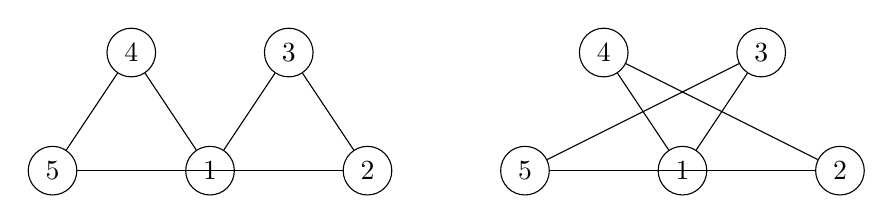
\begin{tikzpicture}
    % Graph A
    \node[shape=circle,draw=black] (1) at (0,0) {1};
    \node[shape=circle,draw=black] (2) at (2,0) {2};
    \node[shape=circle,draw=black] (3) at (1,1.5) {3};
    \node[shape=circle,draw=black] (4) at (-1,1.5) {4};
    \node[shape=circle,draw=black] (5) at (-2,0) {5};

    \draw (1) -- (2);
    \draw (1) -- (3);
    \draw (1) -- (4);
    \draw (1) -- (5);
    \draw (2) -- (3);
    \draw (2) -- (5);
    \draw (4) -- (5);

    % Graph B
    \node[shape=circle,draw=black] (1b) at (6,0) {1};
    \node[shape=circle,draw=black] (2b) at (8,0) {2};
    \node[shape=circle,draw=black] (3b) at (7,1.5) {3};
    \node[shape=circle,draw=black] (4b) at (5,1.5) {4};
    \node[shape=circle,draw=black] (5b) at (4,0) {5};

    \draw (1b) -- (2b);
    \draw (1b) -- (3b);
    \draw (1b) -- (4b);
    \draw (1b) -- (5b);
    \draw (2b) -- (4b);
    \draw (2b) -- (5b);
    \draw (3b) -- (5b);
\end{tikzpicture}



%%%%%%%%%%%%%%%%%%%%%%%%%%%%%%%%%%%%
\section*{Exercise 5 4.1}  

Consider the following two graphs:%
\begin{description}
\item[{\(G_1\)}]\(V_1=\{a,b,c,d,e,f,g\}\)%
\par
\(E_1=\{\{a,b\},\{a,d\},\{b,c\},\{b,d\},\{b,e\},\{b,f\},\{c,g\},\{d,e\}\),%
\par
\(\{e,f\},\{f,g\}\}\).%
\item[{\(G_2\)}]\(V_2=\{v_1,v_2,v_3,v_4,v_5,v_6,v_7\}\),%
\par
\(E_2=\{\{v_1,v_4\},\{v_1,v_5\},\{v_1,v_7\},\{v_2,v_3\},\{v_2,v_6\}\),%
\par
\(\{v_3,v_5\},\{v_3,v_7\},\{v_4,v_5\},\{v_5,v_6\},\{v_5,v_7\}\}\)%
\end{description}
%
\begin{enumerate}[label= (\alph*)]
\item{}Let \(f:G_1 \rightarrow G_2\) be a function that takes the vertices of Graph 1 to vertices of Graph 2. The function is given by the following table:%
\begin{center}
\begin{tabular}{llllllll}
\textbf{x}&\(a\)&\(b\)&\(c\)&\(d\)&\(e\)&\(f\)&\(g\)\\
\hline
\textbf{f (x)}&\(v_4\)&\(v_5\)&\(v_1\)&\(v_6\)&\(v_2\)&\(v_3\)&\(v_7\)
\end{tabular}
\end{center}
%
Does \(f\) define an isomorphism between Graph 1 and Graph 2?%
\item{}Define a new function \(g\) (with \(g \ne f\)) that defines an isomorphism between Graph 1 and Graph 2.%
\item{}Is the graph pictured below isomorphic to Graph 1 and Graph 2? Explain.%
\begin{center}
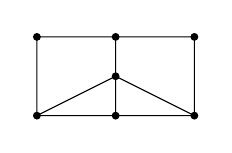
\begin{tikzpicture}
    % Define the vertices as small circles for clarity
    \def\v{circle(0.05) node{}}
	\draw (-1, 0) coordinate (v1) -- (0,0) coordinate (v2) -- (1,0) coordinate (v3) -- (1,1) coordinate (v4) -- (0,1) coordinate (v5) -- (-1,1) coordinate (v6) -- (v1) --(0,.5) coordinate (v7) -- (v2) (v7) -- (v3) (v7) -- (v5);
	\foreach \i in {1,...,7}{
		\fill (v\i) \v;
	}
\end{tikzpicture}
\end{center}
\end{enumerate}

\vspace{0.5cm}
\noindent\textbf{Solution Draft:} 
\vspace{0.2cm}

\begin{enumerate}
    \item[a.] $f$ does not define an isomorphism between Graph 1 and Graph 2. $\{b, c\}$ exists in $G_1$ whereas $\{v_5, v_1\}$ in $G_2$ does not.
    \item[b.] 

    \begin{center}
        \begin{tabular}{llllllll}
        \textbf{x}&\(a\)&\(b\)&\(c\)&\(d\)&\(e\)&\(f\)&\(g\)\\
        \hline
        \textbf{g (x)}&\(v_1\)&\(v_2\)&\(v_3\)&\(v_4\)&\(v_5\)&\(v_6\)&\(v_7\)
        \end{tabular}
        \end{center}

    \item[c.] I believe that it is. It has the 7 verticies and 10 edges and it matches the degrees of $G_1$ and $G_2$
\end{enumerate}

%%%%%%%%%%%%%%%%%%%%%%%%%%%%%%%%%%%%
\section*{Exercise 7 4.1}  

Which of the graphs below are bipartite? Justify your answers.%
\begin{center}
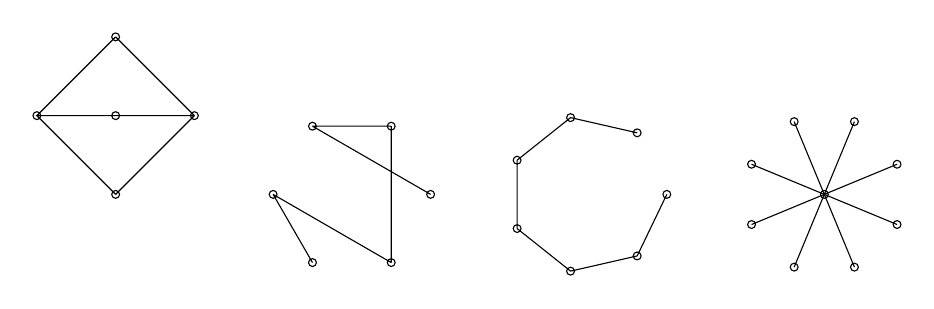
\begin{tikzpicture}
    \def\v{circle(0.05) node{}}
    \begin{scope}[xshift=-3cm]
        \draw (-1,1) \v -- (0,2) \v -- (1,1) \v -- (0,0) \v -- (-1,1) -- (0,1) \v -- (1,1);
    \end{scope}
    \begin{scope}[xshift=0cm]
        \draw (0:1) \v -- (120:1) \v -- (60:1) \v -- (300:1) \v -- (180:1) \v -- (240:1) \v -- cycle;
    \end{scope}
    \begin{scope}[xshift=3cm]
        \draw (360/7:1) \v -- (2*360/7:1) \v -- (3*360/7:1) \v -- (4*360/7:1) \v -- (5*360/7:1) \v -- (6*360/7:1) \v -- (0:1) \v -- cycle;
    \end{scope}
    \begin{scope}[xshift=6cm]
        \draw (0,0) \v;
        \foreach \x in {0,...,7}
            \draw (0,0) -- (\x*360/8+22.5:1) \v;
    \end{scope}
\end{tikzpicture}
\end{center}

\vspace{0.5cm}
\noindent\textbf{Solution Draft:} 
\vspace{0.2cm}

The first graph has an odd number of verticies and forms a closed loop. It is not bipartite

The second graph is a tree. It is bipartite

The third graph is a tree. It is bipartite

The fourth graph is a star graph. It is bipartite because you can bave one set containing the central vertex and the other set containing all the outside verticies.

%%%%%%%%%%%%%%%%%%%%%%%%%%%%%%%%%%%%


\section*{Exercise 14 4.1}  

Consider graphs with \(n\) vertices.  Remember, graphs do not need to be \emph{connected}.%
\begin{enumerate}[label= (\alph*)]
\item{}How many edges must the graph have to guarantee at least one vertex has degree two or more?  Prove your answer.%
\item{}How many edges must the graph have to guarantee all vertices have degree two or more?  Prove your answer.%
\end{enumerate}

\vspace{0.5cm}
\noindent\textbf{Solution Draft:} 
\vspace{0.2cm}

\begin{enumerate}[label= (\alph*)]
    \item You need at least 3 edges to guarantee one vertex has degree two or more.
    
    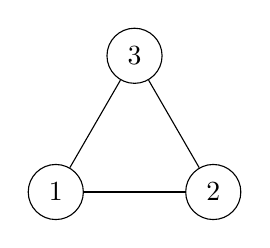
\begin{tikzpicture}
      \node[circle,draw,minimum size=0.7cm] (1) at (0,0) {1};
      \node[circle,draw,minimum size=0.7cm] (2) at (2,0) {2};
      \node[circle,draw,minimum size=0.7cm] (3) at (1,1.73) {3};
      
      \draw (1) -- (2);
      \draw (2) -- (3);
      \draw (1) -- (3);
    \end{tikzpicture}
    \item You need at leat 4 edges to guarantee all vertices have degree two or more.
    
    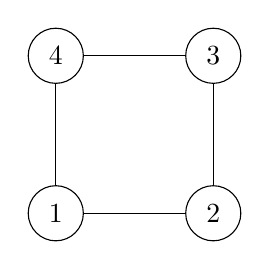
\begin{tikzpicture}
        \node[circle,draw,minimum size=0.7cm] (1) at (0,0) {1};
        \node[circle,draw,minimum size=0.7cm] (2) at (2,0) {2};
        \node[circle,draw,minimum size=0.7cm] (3) at (2,2) {3};
        \node[circle,draw,minimum size=0.7cm] (4) at (0,2) {4};
        
        \draw (1) -- (2);
        \draw (2) -- (3);
        \draw (3) -- (4);
        \draw (4) -- (1);
      \end{tikzpicture}
\end{enumerate}

%%%%%%%%%%%%%%%%%%%%%%%%%%%%%%%%%%%%
\section*{Exercise 3 4.2}  

For each degree sequence below, decide whether it must always, must never, or could possibly be a degree sequence for a tree.  Justify your answers.%
\begin{enumerate}[label= (\alph*)]
\item{}\(\displaystyle (3, 3, 2, 2, 2)\)%
\item{}\(\displaystyle (3, 2, 2, 1, 1, 1)\)%
\item{}\(\displaystyle (3, 3, 3, 1, 1, 1)\)%
\item{}\(\displaystyle (4, 4, 1, 1, 1, 1, 1, 1)\)%
\end{enumerate}

\vspace{0.5cm}
\noindent\textbf{Solution Draft:} 
\vspace{0.2cm}

A tree with $n$ vertices has $n-1$ edges.
A tree is connected and acyclic
The sum of degrees in a tree must equal $2(n-1)$.

\begin{enumerate}[label= (\alph*)]
    \item 
    Sum of degrees $3+3+2+2+2=12$

    Expected sum of a tree with 5 verticies $2*(5-1)=8$

    This sequence must never be a tree.
    \item
    Sum of degrees $3+2+2+1+1+1=10$

    Expected sum of a tree with 6 verticies $2*(6-1)=10$

    This sequence could be a tree.

    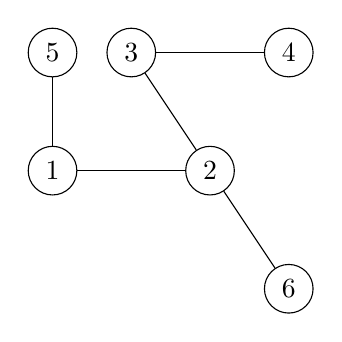
\begin{tikzpicture}
        \node[circle,draw] (1) at (0,0) {1};
        \node[circle,draw] (2) at (2,0) {2};
        \node[circle,draw] (3) at (1,1.5) {3};
        \node[circle,draw] (4) at (3,1.5) {4};
        \node[circle,draw] (5) at (0,1.5) {5};
        \node[circle,draw] (6) at (3,-1.5) {6};
      
        \draw (1) -- (2);
        \draw (2) -- (3);
        \draw (3) -- (4);
        \draw (2) -- (6);
        \draw (1) -- (5);
      \end{tikzpicture}

    \item
    Sum of degrees $3+3+3+1+1+1=12$

    Expected sum of a tree with 6 verticies $2*(6-1)=10$

    This sequence must never be a tree.

    \item
    Sum of degrees $4+4+1+1+1+1+1+1=14$

    Expected sum of a tree with 8 verticies $2*(8-1)=14$

    Even though the number of vertices lines up with the expected number for a tree. Since there are two verticies that are connected to half of the of the verticies, you cannot create this graph without a cycle.

    This sequence must never be a tree.
\end{enumerate}

%%%%%%%%%%%%%%%%%%%%%%%%%%%%%%%%%%%%



\section*{Works cited}
Discrete Mathematics: An Open Introduction, 3rd edition by Oscar Levin.
\end{document}